\documentclass[oneside,11pt]{amsart}
\usepackage[utf8]{inputenc}%
\usepackage[english]{babel}%
\usepackage{amsmath,amssymb,amsthm,amsfonts}%
\usepackage[unicode]{hyperref}%
\usepackage{mathrsfs,bbm}%
\usepackage{paralist}
\usepackage{color}
\usepackage{longtable}
\usepackage{array}
\newcolumntype{L}[1]{>{\small\raggedright\arraybackslash}m{#1}}
\newcolumntype{T}[1]{>{\footnotesize\raggedright\arraybackslash}m{#1}}
\usepackage{stmaryrd}%
%\usepackage{refcheck}
\usepackage{graphicx}
\usepackage[DIV17]{typearea}
\usepackage{multicol,tikz}
\usepackage{datetime}
\usepackage{cleveref}

\usepackage[shadow]{todonotes}

\usepackage{etoolbox}
\patchcmd{\section}{\scshape}{\Large\itshape\bfseries}{}{}

\usepackage{caption}
\captionsetup{labelformat=empty,labelsep=none}

\hypersetup{
  colorlinks=true,
  linkcolor=blue!50!red,
  urlcolor=green!60!black
}

%%%%%%%%%%%%%%%%%%%%%%%%%%%%%%%%%%%%%%%%%%%%%%%%%%%%%%%%%%%%%%%%%%%%%%%%%%%%%%%%%%%%%%%%
\synctex=1
%%%%%%%%%%%%%%%%%%%%%%%%%%%%%%%%%%%%%%%%%%%%%%%%%%%%%%%%%%%%%%%%%%%%%%%%%%%%%%%%%%%%%%%%
%%%%%%%%%%%%%%%%%%%%%%%%%%%%%%%%%%%%%%%%%%%%%%%%%%%%%%%%%%%%%%%%%%%%%%%%%%%%%%%%%%%%%%%%
\newcommand{\score}[1]{\textit{#1}\addtocounter{totalscore}{#1}}
\newcommand{\razdel}[1]{\smallskip\underline{\textbf{#1:}}\smallskip}

\newcommand{\note}[1]{{\sf{}\color{blue}(#1)}}

\begin{document}

\title[MATH 3100: INTRODUCTION TO PROBABILITY]{MATH 3100: INTRODUCTION TO PROBABILITY}
\author{Leonid Petrov\\Fall 2022\\Sections 001, 002, and 003}
\date{Compiled on \today, \currenttime.\\An up to date syllabus is always on \texttt{GitHub} at \url{https://github.com/lenis2000/Syllabi/blob/master/Syllabus_3100_s22.pdf}. For direct PDF download use \href{https://github.com/lenis2000/Syllabi/raw/master/Syllabus_3100_s22.pdf}{\texttt{this link}}.
	\LaTeX{} source with \textit{changes} to the syllabus is \href{https://github.com/lenis2000/Syllabi/blob/master/Syllabus_3100_s22.tex}{\texttt{here}}
(click ``History'').}
\maketitle

\bigskip

$\boxed{\textnormal{IMPORTANT: CLASSES AND OFFICE HOURS ARE ONLINE UNTIL FEBRUARY 4, 2022}}$


\section{A mathematical study of randomness}

How random is everything around us, and what chance do we have of understanding it? What to do when you're not certain, and how to do it right? How many falling stars will you see as you walk outside one beautiful night? 

Probability theory is a mathematical study of uncertainty. It is a rigorous foundation of statistics --- and many areas of human knowledge operate in a language of statistics nowadays (yes, and robots use it, too!). The course introduces fundamental concepts, ideas, and techniques of probability theory. It will provide you with the foundational mathematical knowledge needed to address the questions above and will help you develop intuition about randomness.


\begin{figure}[h]
	\begin{tabular}{ccc}
		
\includegraphics[height=.32\textwidth]{img/Bond_percolation_p_51.png}
		&\hspace{10pt}
\includegraphics[height=.32\textwidth]{img/Amas_de_percolation_gray.png}
		&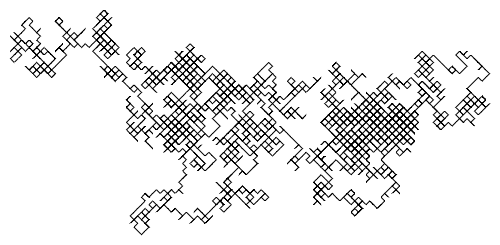
\includegraphics[angle=90,height=.32\textwidth]{img/RW1.png}
	\end{tabular}
	\def\figurename{}
	\caption{Examples of random structures: bond percolation
	\href{https://en.wikipedia.org/wiki/Percolation_theory}{\texttt{close-up}}
	(left),
	at a \href{https://commons.wikimedia.org/wiki/File:Amas_de_percolation.png}{\texttt{larger scale}} (center),
	and
	a 
	\href{https://en.wikipedia.org/wiki/Random_walk\#Lattice_random_walk}{\texttt{random walk}}
	(see also a
	\href{https://upload.wikimedia.org/wikipedia/commons/f/f3/Random_walk_2500_animated.svg}{\texttt{simulation}} 
	of a random walk).
	\tiny{Note:
	this PDF has green clickable links, like in the previous sentence.}
	}
\end{figure}

\subsection*{What you will get from this course}

\begin{enumerate}[\bf{}1.]
	\item Mastery of basic probability concepts:
	\begin{enumerate}[(a)]
		\item What is a probability space and how to translate commonly-sounding problems into this language;
		\item How to count (in an advanced way) to compute probabilities;
		\item What is a random variable, a probability distribution,
		and what are their main quantitative properties;
		\item 
		How commonly encountered probability 
		distributions (binomial, Poisson, exponential, Gaussian) look like and behave,
		what are 
		their properties, and in which situations they typically arise.
	\end{enumerate}

	\item How large random systems behave, and what the 
	bell-shaped curve
	\raisebox{-8pt}{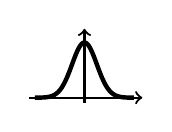
\begin{tikzpicture}
		[scale=.7]
		\draw[ultra thick, domain=-.9:.9] plot[samples=300] ({\x}, {2.7128^(-10*\x*\x)});
		\draw[->, thick] (-1.01,0)--(1.05,0);
		\draw[->, thick] (0,-.1)--(0,1.25);
	\end{tikzpicture}}
	has to do with this.
	\item How to describe and quantify the mutual dependence of random events,
	and how to use such a description 
	to infer properties of ``hidden'' random events.
	\item How to apply probability theory to model real-life processes. For example,
		how to use Bayes theorem to understand various medical tests.
	\item How to collaborate on solving probability problems in pairs, small groups, and online,
	and present solutions clearly and efficiently.
	% \item How to design probability problems (for example, for the
	% final exam), and evaluate problems presented by others.
	\item In what ways probability theory is connected to science,
	engineering, and other branches of knowledge.
\end{enumerate}

\subsection*{Prerequisite} You should have taken at least one semester of calculus (MATH 1320 level):
mathematical study of random variables often requires single and double integrals
and infinite series.

\subsection*{What this course is and what it is not}

This course in probability \emph{theory} belongs to pure mathematics, with
rigorous definitions, calculations, and proofs. However, the objects which we
study are motivated by real-life applications, and so pure mathematical
arguments often appeal to our common sense understanding of these objects.
There will be opportunities to explore (and discover new) connections of the
theory studied in the course with the real world.

Also, this course does not thoroughly discuss \emph{applications to statistics}.
Probability
theory focuses on developing the mathematical side, and statistics applies
these mathematical theories to real data (coming from observations). In this
course we will not discuss how to analyze data coming from observations ---
there are courses in statistics for that.

\section{Necessary information}
\label{sec:necc}

\subsection{Meeting times}{\ }\\
\label{sub:meeting_times}

\begin{tabular}{|r|l|l|l|}
	\hline
	&Section 001
	&Section 002
	&Section 003
	\\
	\hline
	\rule{0pt}{34pt}
	\parbox{.2\textwidth}{\textbf{Class times}\\
	January 19\\\qquad  --- May 3}
	& \parbox{.22\textwidth}{MWF, Monroe 118\\ 10:00AM - 10:50AM\\ (on Zoom till Feb 4)}
	& \parbox{.22\textwidth}{MWF, Monroe 118\\ 11:00AM - 11:50AM\\ (on Zoom till Feb 4)}
	& \parbox{.22\textwidth}{MWF, Monroe 118\\ 12:00PM - 12:50PM\\ (on Zoom till Feb 4)}
	\\[8pt] \hline
	\textbf{Midterm 1}   
	& February 18
	& February 18
	& February 18
	 \\ \hline
	 \textbf{Midterm 2}   
	 & March 30
	 & March 30
	 & March 30
	 \\ \hline
	 \textbf{Final exam}     
		& Date TBA	
		& Date TBA	
		& Date TBA	
	 \\ \hline
\end{tabular}

\bigskip

\textbf{Instructor:} Leonid Petrov, Kerchof 209

	\textbf{Questions to the instructor:} We use \texttt{Slack}, see \Cref{comm}

	\textbf{Office hours:} 
	Mondays and Wednesdays at 2:30PM-3:30PM; and by appointment $\downarrow$
	
	You can automatically schedule an office hours appointment 
	at \href{https://lpetrov.cc/teaching/}{\texttt{this page}} (you don't need an appointment for 
	regular office hours).
	You can make as many appointments as you need throughout the semester. Each appointment
	must be made at least 3 hours prior to the time of the appointment.

	Office hours occur in Kerchof 209. Office hours by appointment
	could meet in zoom, too.
	
\subsection{About the instructor}
I am an Associate Professor in the Department of Mathematics at UVA, and I've
been here since 2014. My research area is probability theory (very appropriate
for this course!). More precisely, I am using exact formulas to study large
random systems. I also like computer simulations of random systems like 
\href{https://d3m0khvr0ybm92.cloudfront.net/img/blog/heart/UVA_colors_small.png}{\texttt{this one}}.
I'm happy to tell you more if you're
interested.

\subsection{Textbook}
\label{sub:main_textbook}

Anderson, Sepp\"al\"ainen, Valk\'o, \emph{Introduction to Probability}, 1st Edition.

ISBN-13: 978-1108415859; 
ISBN-10: 9781108415859.

See also \Cref{success} below for discussion 
of how we'll use the textbook,
and for other helpful resources.

\subsection{Inverted format}

\begin{itemize}
	\item \textbf{Lectures} are pre-recorded and are uploaded to Panopto (collab $\to$ lecture capture). 
		Watching lectures (live or recorded) is required as 
		a part of the homework.
		Each lecture has a date, and this is the date by which you should watch the lecture.

		A summary of the lectures content is posted at 
		\url{https://github.com/lenis2000/Math3100_S22_LectureNotes/blob/main/lecture_notes.pdf})
		(\href{https://github.com/lenis2000/Math3100_S22_LectureNotes/raw/main/lecture_notes.pdf}
		{\texttt{link to automatically download}}).

		
	\item \textbf{In class}, I briefly review the material of the lectures
		and answer your 
		questions. There are also occasional pop quizzes.
		However, most of the class time is spent on \textbf{problem solving}.
		That is, you are going to work together 
		on this week's problem set (that is also at the same time this week's homework).
		That is, we are \emph{doing homework in class}.
		Ideally, after the class you just need to write up your solutions 
		and submit on collab. 
		Participation and active role in class work 
		will be rewarded by points towards the final grade.
\end{itemize}

Note for class meetings till February 4: These zoom meetings are 
dedicated to discussion, and are \textbf{not recorded}.

\subsection{Checklist to start participating in the class}

Since classes and office hours are online until February 4, 2022, here is a checklist to start:
\begin{enumerate}
	\item Join the Collab website called \textbf{MATH3100 S22}.
	\item Use the slack join link to join the course slack space.
	\item View the short introduction video
	\item Come to your section's zoom meeting on January 19, and subsequently to all 
		meetings on Mondays, Wednesdays, and Fridays. The zoom links are on Collab.
\end{enumerate}
See you in person on February 7 in Monroe 118.

\section{Assessing your learning}

Learning mathematics means \emph{doing} mathematics: during class meetings, on your own, and in groups.
In this course, doing mathematics mainly amounts to solving problems.
The following aspects are assessed in this course:

\subsection{Course engagement (15\%)}

I am putting a lot of emphasis
into the various engagement components which ask you to interact with 
your peers (and the instructor) while learning the material. This includes:\footnote{It is 
hard to predict how the categories below are going to be weighted relatively to each other
depending on the amount of activity throughout the semester; but they sum up to 25\% in total.}

\begin{itemize}
	\item \textbf{Slack}. Ask questions about the class, and answer others' questions.
	\item \textbf{In-class participation}. 
		Being present and involved in discussions at most of the in-class meetings
		is essential to getting a hands-on experience 
		in problem solving. 
		I understand that many people cannot participate in all class meetings due to various
		circumstances. 
		If needed,
		you can occasionally come to meetings of another section (see \Cref{sub:another_section_going}
		for restrictions on that).
		I expect to give full credit for class participation 
		if you come to at least 75\% of the class meetings (not counting midterms).
	\item \textbf{Quizzes}. 
		Prior to each class, you are expected to have watched the corresponding recorded lecture.
		(Each lecture on Panopto is dated with the date you should watch it by.)
		There will be occasional pop quizzes in class,
		to make sure you are paying attention to the material. 
		Lowest $x$ quiz grades is dropped from the calculation (here $x=1$ or $2$, depending
		on the total number of quizzes we end up having).
	\item \textbf{Office hours}. Come to office hours (if needed, 
		sing up for appointments, see \Cref{sub:meeting_times}) 
		with questions about problem sets and recorded lectures.
		I am always happy to discuss your ideas and explain math.
		As a rule, I expect every student to come to office hours or schedule a one on one appointment
		at least once throughout the semester.
\end{itemize}

I expect that most people who are paying attention to the class,
come to meetings, and interact with peers, will get close to full credit for
the course engagement.

\subsection{Problem sets (30\%; lowest problem set grade is dropped)}

\begin{enumerate}[$\bullet$]
	\item Weekly problem sets consist of textbook and other problems aligned with lectures, to
		help you practice new concepts and techniques. 
		The written solutions are due on
		Mondays at 10pm
		(except weeks with midterms).
		Problem sets are posted to Collab assignments
		at least one week in advance.
		You will be working on them during the discussion times in class meetings.
	\item You are encouraged to work together on problem sets in the off-times, too,
		in slack (you may create private groups there; ask me if you need more permissions),
		and by any other means of communication, or in person.
		Group work allows to 
		take advantage of challenge-defend discussions which help understand things
		better.
		However, each student needs to submit her/his own written work, 
		and should write this up individually. 
		This helps better retain the material and prepare for tests.
	\item The written solutions are graded ``coarsely'', that is,
		each problem set will be assigned one of four grades: 
		\begin{equation*}
			\begin{tabular}{l|l|l|l|l}
				Grade & VG (very good) & G (good) & OK   & N \\
				\hline
				& \parbox{.21\textwidth}{All problems solved correctly with minor issues like arithmetic mistakes, and solutions explained
				in full detail}
				& \parbox{.21\textwidth}{Most problems solved correctly, and solutions explained in reasonable (close to full) detail}
				& \parbox{.21\textwidth}{ {\ }\\More than $3/4$ of problems attempted, many 
				solutions are incorrect, incomplete, or not explained in detail, 
				but the work displays adequate understanding of most of the material\\{}}
				& \parbox{.21\textwidth}{Work not submitted on time, or less than $3/4$ of problems 
				attempted, or most solutions are incomplete, or work clearly displays lack of understanding of most of the material}\\
				\hline
				\%    & 100\%          & 90\%     & 75\% & 0\%
			\end{tabular}
		\end{equation*}
		It is expected that most students 
		who put reasonable effort into the work
		will get VG or G grades. 
	\item 
		The work \emph{must be submitted only on Collab} --- 
		take pictures or scan your work,
		make sure it's readable,
		put it into a \emph{single PDF file with correct orientation},
		and upload it to the Collab assignments before the deadline.
		Failure to make a single PDF might result in zero points for a work
		(first, a warning will be given).
\end{enumerate}

When solving homework problems, use your math and common sense understanding to check for your own mistakes,
see \Cref{sub:problem_solving} for details.

\subsection{Midterm tests (2 tests each worth 15\%; 30\% in total)}

There are two midterm tests
held
during regular class times, on \textbf{February 18} and \textbf{March 30}.
They have
similar taste as homework, and test basic knowledge of the material.

A two-sided letter size formula sheet, hand-written by yourself, is
allowed on each midterm test and on the final exam. Preparing this formula sheet
will help you review the material, and paint a systematic picture of the material in your mind.
Formula sheets cannot contain any photocopied or printed material
--- do everything by hand (of course, you can include any theorems, formulas, pictures, 
examples, etc).
The use of calculators (but not in mobile phones)
is allowed on the midterm tests and the final exam.

I encourage you to collaborate on preparing for the tests, but needless to say that
during the test and the final exam each student must work individually.

When solving midterm problems, use your math and common sense understanding to check for your own mistakes,
see \Cref{sub:problem_solving} for details.


\subsection{Final exam (25\%)}

The final exam will be cumulative, but will put more focus 
on topics covered after the second midterm.
Formula sheet is also allowed, same as for midterms.

On the final exam, use your math and common sense understanding to check for your own mistakes,
see \Cref{sub:problem_solving} for details.


\subsection*{Letter grades}

The scale by which course percent grades are turned into course letter grades
will most likely be the following:
\begin{equation*}
	\begin{tabular}{l|l|l|l|l|l|l|l|l|l|l|l|l|}
		Grade      & $ A+	$ & $A	$ & $A-	$ & $B+	$ & $B	$ & $B-	$ & $C+	$ & $C	$ & $C-	$ & $D+	$ & $D	$ & $D-$ \\
		\hline
		Minimum \% & 100     & 93   & 89    & 86    & 82    & 79    & 76    & 72    & 69    & 66    & 62    & 59
	\end{tabular}
\end{equation*}
I reserve the right to slightly change this grade scale after the
final exam.
This may be needed
to better incorporate into the letter grade
possible fluctuations in the difficulty level of 
midterms and the final.

\section{Communication}
\label{comm}

\subsection{Email}
\label{sub:email}

My email address is \href{mailto:petrov@virginia.edu}{petrov@virginia.edu}.
This is a backup channel for communication in case slack or collab fails.
In general, you have to
ask your mathematical questions (and questions about the course) on slack.

\subsection{Slack}
\label{sub:slack}

This is the space to ask (and answer!) 
questions about problem sets, 
lectures, and anything related to the course. The aim of slack is to build a community of learners
of probability theory.

Slack is an
industrial standard of work messengers, with a web version and apps for all
platforms. This will make me more accessible if you have questions, and also
will let you answer questions of your fellow students.

The link to sign up to the slack space for the course is found on collab.
Please
let me know if you have issues with access. 
It is also expected that you
will check announcements, and will participate in (or at least read)
most of the discussions of the course material.

Some things to note: 
\begin{enumerate}[$\bullet$] 
	\item \textbf{Population}:
		The \texttt{Slack} team will contain of students
		of all 3 sections of MATH3100 this semester, which is 
		around 120 students.
	\item \textbf{Direct messages}:
		Direct messages are an excellent tool in \texttt{Slack} to communicate
		with me. When sending your very first direct message to me, please 
		write your full name and which section you're from (if this is not obvious from your nickname).
	\item \textbf{Direct messages to other students}:
		There are direct messages where you can talk to other students
		one-on-one. 
		You can also create private groups with up to 9 people, which
		is good for homework collaboration (but read \Cref{collaboration} on
		collaboration).
	\item \textbf{Privacy}:
		Although \texttt{Slack} is a messaging app, it should be used
		professionally, especially in public discussions. The app supports private
		direct and group messages. But please note that in principle the admin
		(i.e., myself) can obtain access to \textbf{all} direct messages between
		members of the team. 
		I assure you that this may be done only in extreme circumstances.
	\item \textbf{Notifications}:
		With \texttt{Slack}, it is easy to not miss important announcements and direct messages, 
		even if 
		you don't check it all the time --- 
		under the default settings, you will get notified (by email, too)
		about direct messages and mentions of your name. 
		All announcements will have mentions of everybody
		to draw attention. 
		Also, you can change notification settings, but please remember that
		there will be sometimes very important activity in \texttt{Slack} that you don't want to miss.
	\item \textbf{Many other features}: 
		\texttt{Slack} supports reminders out of the box. 
		You can ask it to remind yourself about a particular message, or 
		just set a general reminder. 
		With this, it is 
		easy to keep track of important messages
		(like class announcements or problems I'll post there).
\end{enumerate}

The slack space is separated into channels:
\begin{itemize}
	\item 
		\#hw-01, \ldots,  \#hw-10 for homeworks
	\item 
\#midterm-1, \#midterm-2 for midterms 
\item 
\#final for the final exam
\item 
\#lectures for lecture announcements and questions, 
\item 
\#questions for any other questions you might have, including general discussion.
\item 
\#general is for general announcements and I will keep only the most necessary things here.
\item 
\#introductions if you’d like to write a couple of words about yourself - I’m curious to meet and get to know you all!
(Except \#introductions, all other channels include everybody by default.)
\end{itemize}

\subsection{Zoom class meetings (till February 4)}

I will have my camera on during Zoom sessions, and invite you to keep
your camera on if you are comfortable doing so. Whether or not your
camera is on, your active participation in the course is essential.
Please show initiative, active listening, and courtesy through the
following: 
\begin{itemize}
	\item 
Use the chat to ask questions, report problems, or whenever directed as part of a class activity. Keep chat messages respectful, concise, and relevant. I’m not judging your grammar, but remember you’re writing in an academic environment, even in the chat box. 
\item 
Use the ‘reactions’ buttons (clapping, thumbs up) if appropriate!
\item 
Keep your mic muted when you aren’t speaking, to lessen distractions (and forgive me if I occasionally have to mute you if you forget).
\item 
	Unmute yourself to ask questions when I am speaking; alternatively,
	use the ‘raise hand’ button.
\item 
Remember that when two people talk at the same time in Zoom, neither can be easily heard. 
So leave time between speakers.
\item 
In this online environment, I will probably ‘cold call’ students more often than I would in the classroom. It can be hard for me to know who is ready to speak, so I may call on you when you’re not expecting it. If you need to ‘pass’ on a question once or twice, that’s OK.
\end{itemize}

\subsection{Collab anonymous feedback}
\label{sub:collab}
If you have anonymous comments on anything related to the course, you can make
them via Collab.

\section{How to succeed in the course}
\label{success}

If you read the long syllabus through here, you are on the right
track to succeed!

\subsection{General things}

The best way to learn in the course is to 
watch all recorded lectures and take notes to retain the material in memory; 
come to all classes;
and do all the homework problems on your own or in collaboration.
This will prepare you well for tests.

\subsection{Main textbook}

The textbook \emph{Introduction to Probability} by Anderson, Sepp\"al\"ainen, and Valk\'o 
is 
an excellent resource 
to gain understanding of the course material. Some notes about it:

\begin{enumerate}[$\bullet$]
	\item I strongly encourage you to read the textbook in parallel with watching the lectures, as lectures are largely based on the textbook.
		The textbook includes many examples and
		extra exercises which augment the concepts discussed in class.
	\item The textbook contains much more material than will be covered in classes, so it
		makes sense to watch lectures and come to classes to note which parts are omitted
		(and so won't be in tests).
\end{enumerate}

\subsection{Additional textbooks}

\begin{enumerate}
	\item 
		\emph{``Probability'' by Jim Pitman} is a reasonable alternative textbook.
	\item 
		\emph{Free textbook} 
		\emph{``Introduction to Probability'' by Grinstead and Snell}.
			Download: \url{https://math.dartmouth.edu/~prob/prob/prob.pdf};
			Accompanying web page: \url{https://www.dartmouth.edu/~chance/teaching_aids/books_articles/probability_book/book.html}.
\end{enumerate}

These textbooks contain additional problems and material.
They may be helpful if you want a deeper understanding of
some concepts, or if you want to read an exposition of the
familial material in a different style, which might be very
helpful for better learning.

(It absolutely not required that you buy or read these books.)

\subsection{Problem solving and self-checking}
\label{sub:problem_solving}

Solving problems, one can easily make arithmetic mistakes,
and this is understandable. However, 
we are doing probability theory, so some answers to problems
may be easily dismissed as wrong
based on common sense. 
The most obvious examples are 
getting a \emph{negative probability}; \emph{probability strictly greater than 1};
getting a \emph{negative variance}; and so on.
It is expected that you use this type of common sense to filter out 
obviously wrong answers.
Solid partial credit will be given even in the case when you get an obviously
wrong answer, and note near it:
\begin{quote}
	``Well, this answer is clearly incorrect because $\{\textnormal{expanation}\}$''.
\end{quote}
Obviously wrong answers without such a note 
will result in much less partial credit for the whole problem.

\subsection{Extra reading}

The popular book
\emph{``How Not to Be Wrong: The Power of Mathematical Thinking'' by Jordan Ellenberg}
discusses how math touches every aspect of real life, and has 
numerous examples related to probability and statistics. 
I can recommend this nice book as a parallel reading. Some
examples I learned from this book might be mentioned in class.
(It absolutely not required that you buy or read this book.)

\subsection{Slack}

Ask mathematical questions about homework, lectures, and anything else
related to the class on Slack 
(see \Cref{sub:slack}).
Answer other students' questions.

\subsection{Office hours}

I am available during office hours to answer questions on the content of the 
course, clarify various points, and I can also help you with homework assignments. 
Besides regular office hours, you can automatically schedule appointments, see 
\Cref{sec:necc}.

\subsection{Math Collaborative Learning Center}

The Math Department 
Collaborative Learning Center
is available for helping students in this course: 
see \url{https://math.virginia.edu/undergraduate/MCLC/}
for more information and schedule. 
(Usually it takes a week or so after the semester starts for MCLC to start working.)

\subsection{Other resources}

There is a number of online resources which may help you while doing the homework:
Khan Academy, Wikipedia, and many other 
places contain lots of basic material on probability theory. Google Search
in general
is also a valuable resource.

\subsection{Collaboration on homework assignments}
\label{collaboration}

Group work on homework problems is allowed and strongly encouraged.
Discussions are in general very
helpful and inspiring. Class meetings will also contain ample time
for group work on homework problems.
Nevertheless, before talking to others, get well started
on the problems, and contribute your fair share to the process. 

When completing the written homework assignments, everyone must write up his or her own
solutions in their own words, and cite any reference 
(other than the textbook and
class notes) that you use. Quotations and citations are part of the Honor Code for both UVa
and the whole academic community. 

It is very important that you truly understand the homework solutions you hand
in, otherwise you may be unpleasantly surprised by your test results.

\section{Approximate course schedule}

\noindent Add/drop information: \href{https://registrar.virginia.edu/enrollment-information/spring-2022-enrollment-instruction}{\texttt{see here}}.
\bigskip

\begin{quote}
	The course has 3 ``pillars'': central limit theorem for Gaussian approximation, 
	Poisson processes, and conditional expectations. 
	Plus there are several technical things to learn: random variables, expectations as integrals, 
	joint distributions, etc.
\end{quote}

\bigskip

A summary of the lectures content is posted at 
\url{https://github.com/lenis2000/Math3100_S22_LectureNotes/blob/main/lecture_notes.pdf})
(\href{https://github.com/lenis2000/Math3100_S22_LectureNotes/raw/main/lecture_notes.pdf}
{\texttt{link to automatically download}}).

\bigskip

All sections are from the main textbook (\Cref{sub:main_textbook}):
\begin{enumerate}[\bf{}{[}week 1{]}]
	\item 1/19, 1/21.
		Introduction. Sample space, axioms of probability, random sampling, review of counting 
		(\texttt{1.1-1.2}).
	\item 1/24, 1/26, 1/28.
		Problem set 1 (shortened) due on Monday.
		Infinitely many outcomes. Geometric series. 
		Rules of probability, Venn diagrams, random variables
		(\texttt{1.3-1.5}).
	\item 1/31, 2/2, 2/4.
		Problem set 2 due on Monday.
		Conditional probability, Bayes' formula, independence
		(\texttt{2.1-2.3}).
	\item 2/7, 2/9, 2/11.
		Problem set 3 due on Monday.
		Independent trials, birthday problem, conditional independence, 
		probability distribution of a random variable
		(\texttt{2.4-2.5, 3.1}).
	\item 2/14, 2/16, \textbf{2/18} (\textbf{Midterm 1}).
		Problem set 4 due on Monday.
		Probability distribution of a random variable,
		cumulative distribution function (\texttt{3.1-3.2}).
	\item 2/21, 2/23, 2/25.
		No problem set due on Monday.
		Cumulative distribution function, 
		expectation, variance, 
		Gaussian distribution
		(\texttt{3.3-3.5}).
	\item 2/28, 3/2, 3/4.
		Problem set 5 due on Monday.
		Gaussian distribution, normal approximation,
		law of large numbers
		(\texttt{3.5, 4.1-4.2}).
		Applications of normal approximation (\texttt{4.3}).
	\item 3/14, 3/16, 3/18.
		Problem set 6 due on Monday.
		Poisson approximation, exponential distribution, Poisson process
		(\texttt{4.4-4.6}).
	\item 3/21, 3/23, 3/25.
		Problem set 7 due on Monday.
		Poisson process, gamma distribution (\texttt{4.6}). 
		Joint distributions (\texttt{6.1-6.3}).
	\item 3/28, \textbf{3/30} (\textbf{Midterm 2}), 4/1.
		Problem set 8 (shortened) due on Monday.
		Joint distributions (\texttt{6.1-6.3}).
	\item 4/4, 4/6, 4/8.
		No problem set due.
		Sums of independent random variables and related topics (survey of 
		selected material of chapters \texttt{7} and \texttt{8}).
	\item 4/11, 4/13, 4/15.
		Problem set 8 due on Monday.
		Law of large numbers, central limit theorem (\texttt{9.1-9.3}).
	\item 4/18, 4/20, 4/22.
		Problem set 9 due on Monday.
		Conditional distributions (\texttt{10.1-10.3}).
	\item 4/25, 4/27, 4/29.
		Problem set 10 due on Monday.
		Conditional distributions (\texttt{10.1-10.3}).
	\item 5/2.
		Problem set 11 due on Monday.
		Overview of cutting edge research in Probability Theory.
\end{enumerate}

\section{Policies}

\subsection{Going to another section's meeting}
\label{sub:another_section_going}

I teach three sections of MATH3100 this semester, with identical content
except for quizzes, tests, and exams.
In general, \textbf{you should come to class at your assigned section's time}
(that is, switching sections on a regular basis is not allowed).
However, occasionally when you have a schedule conflict,
you can come at another section's time. Occasionally means 3-5 times 
during the semester. 
There are also the following caveats:
\begin{itemize}
	\item 
		Coming to a different section time must not exceed classroom's capacity
		(capacity does not matter for zoom meetings which are till February 4).
	\item You must come at \textbf{your assigned section time} for 
		all midterms and the final exam
		(unless you arrange with me otherwise 
		before the midterm / exam).
\end{itemize}


\subsection{Late/make up work} Each assignment will have due date and time.
Late assignments are not accepted. There will also be no make up for the midterm test.
However, if you have special needs, emergency, or unavoidable conflicts, please
let me know as soon as possible, so we can arrange a workaround.
A workaround may include an extra homework which would repair some of the grade.

\subsection{Special needs}

All students with special needs requiring accommodations should present the
appropriate paperwork from the Student Disability Access Center (SDAC). It is
the student's responsibility to present this paperwork in a timely fashion and
follow up with the instructor about the accommodations being offered.
Accommodations for test-taking (e.g., extended time) should be arranged at
least 5 business days before an exam.

\subsection{Honor Code} The University of Virginia Honor Code applies to this
class and is taken seriously (in particular, 
see \Cref{collaboration} on homework collaboration).
Any honor code violations,
especially in written tests (midterms and the final exam)
will be referred to the
Honor Committee.

\subsection{Recording}

The lectures are recorded and posted to Panopto 
(collab $\to$ lecture capture).
Per University of Virginia
policies,
these recordings cannot be shared outside of our course.












\end{document}
